\documentclass{oblivoir}
\usepackage{amsmath,amssymb,amsthm,kotex,paralist,kswrapfig}

\usepackage[skipabove=10pt]{mdframed}

\usepackage{tabto,pifont}
\TabPositions{0.2\textwidth,0.4\textwidth,0.6\textwidth,0.8\textwidth}
\newcommand\tabb[5]{\par\noindent
\ding{172}{#1}
\tab\ding{173}{#2}
\tab\ding{174}{#3}
\tab\ding{175}{#4}
\tab\ding{176}{#5}}

\usepackage{enumitem}
%\setlist{noitemsep}
\setlist[enumerate]{label=(\arabic*)}

\newcounter{num}
\newcommand{\defi}[1]
{\bigskip\noindent\refstepcounter{num}\textbf{정의 \arabic{num}) #1}\par\noindent}
\newcommand{\theo}[1]
{\bigskip\noindent\refstepcounter{num}\textbf{정리 \arabic{num}) #1}\par\noindent}
\newcommand{\exam}[1]
{\bigskip\noindent\refstepcounter{num}\textbf{예시 \arabic{num}) #1}\par\noindent}
\newcommand{\prob}[1]
{\bigskip\noindent\refstepcounter{num}\textbf{문제 \arabic{num}) #1}\par\noindent}
\newcommand{\proo}
{\bigskip\textsf{증명)}\par}

\newcommand{\ans}{
{\par
\raggedleft\textbf{답 : (\qquad\qquad\qquad\qquad\qquad\qquad)}
\par}\bigskip\bigskip}
\newcommand{\procedure}[1]{\begin{mdframed}\vspace{#1\textheight}\end{mdframed}}

\newcommand{\pb}[1]%\Phantom + fBox
{\fbox{\phantom{\ensuremath{#1}}}}

\newcommand\ov[2]{\ensuremath{\overline{#1#2}}}

%%%%
\begin{document}

\title{윤영 : 12 등비수열}
\author{}
\date{\today}
\maketitle
\tableofcontents
\newpage

%%
\section{등비수열의 일반항}

다음과 같은 수열 \(\{a_n\}\)을 생각하자.

\bigskip
\(1\quad3\quad9\quad27\quad81\quad243\quad729\) \tab\tab\(\cdots\cdots\quad \{a_n\}\)

\bigskip\noindent
이 수열은 항 사이의 비가 3으로 일정하다;
\[\frac{a_2}{a_1}=3,\quad \frac{a_3}{a_2}=3,\quad \frac{a_4}{a_3}=3,\quad \frac{a_5}{a_4}=3,\quad \frac{a_6}{a_5}=3,\quad \quad\cdots\]

이처럼, 인접한 항 사이의 비가 일정한 수열을 \textbf{등비수열}이라고 부른다.
이때, 등비수열에서 인접한 항 사이의 비를 \textbf{공비}라고 부른다.
공비는 보통 \(r\)로 쓴다.

%
\begin{mdframed}[innertopmargin=-5pt]
\defi{등비수열}
수열 \(\{a_n\}\)이 다음 조건을 만족시키면 이 수열은 등비수열이다.
\[\frac{a_{n+1}}{a_n}=r.\quad(n\text{은 자연수})\]
\end{mdframed}
%
\prob{}
다음 수열들 중 등비수열인 것을 고르고, 등비수열인 경우 공차 \(r\)를 구하여라.
\begin{enumerate}
\item
\(1\quad3\quad5\quad7\quad9\quad11\quad13\)
\tab\qquad\qquad등비수열이다/아니다 : \(r=\pb{11}\)
\item
\(2\quad4\quad8\quad16\quad32\quad64\quad128\)
\tab\qquad\qquad등비수열이다/아니다 : \(r=\pb{11}\)
\item
\(3\quad6\quad12\quad24\quad48\quad96\quad192\)
\tab\qquad\qquad등비수열이다/아니다 : \(r=\pb{11}\)
\item
\(5\quad5\quad5\quad5\quad5\quad5\quad5\)
\tab\qquad\qquad등비수열이다/아니다 : \(r=\pb{11}\)
\item
\(1\quad-1\quad1\quad-1\quad1\quad-1\quad1\)
\tab\qquad\qquad등비수열이다/아니다 : \(r=\pb{11}\)
\item
\(8\quad4\quad2\quad1\quad\frac12\quad\frac14\quad\frac18\)
\tab\qquad\qquad등비수열이다/아니다 : \(r=\pb{11}\)
\item
\(10\quad100\quad1000\quad10000\quad100000\)
\qquad\quad\:등비수열이다/아니다 : \(r=\pb{11}\)
\item
\(9\quad99\quad999\quad9999\quad99999\)
\tab\qquad\qquad등비수열이다/아니다 : \(r=\pb{11}\)
\item
\(8\quad4\sqrt2\quad4\quad2\sqrt2\quad2\quad\sqrt2\quad1\)
\tab\qquad\qquad등비수열이다/아니다 : \(r=\pb{11}\)
\end{enumerate}

%
\prob{}\label{geometric_example}
다음 등비수열의 여섯 번째 항을 구하여라.
\begin{enumerate}
\item
\(\{a_n\}:2\quad4\quad8\quad\cdots\)
\item
\(\{b_n\}:2\quad6\quad18\quad\cdots\)
\item
\(\{c_n\}:1\quad-1\quad1\quad\cdots\)
\item
\(\{d_n\}:6\quad3\quad\frac32\quad\cdots\)
\item
\(\{e_n\}:4\quad-2\quad1\quad\cdots\)
\end{enumerate}

%
\prob{}
문제 \ref{geometric_example}에 제시된 등비수열의 일반항을 구하여라.
\begin{enumerate}
\item
\(a_n=\)
\item
\(b_n=\)
\item
\(c_n=\)
\item
\(d_n=\)
\item
\(e_n=\)
\end{enumerate}

\clearpage
%
\begin{mdframed}[innertopmargin=-5pt]
\theo{}
첫번째 항(=\(a_1\))이 \(a\)이고 공비가 \(r\)인 등비수열의 일반항은
\[a_n=ar^{n-1}\]
이다.
\end{mdframed}

\proo
첫번째 항이 \(a\)이고 공비가 \(r\)인 등비수열의 항을 나열해보면
\begin{align*}
a_1&=a\\
a_2&=a_1\times r=ar\\
a_3&=a_2\times r=ar^2\\
a_4&=a_3\times r=ar^3\\
a_5&=a_4\times r=ar^4\\
&\vdots
\end{align*}
이다.
따라서
\[a_n=ar^{n-1}\]
이다.
\qed

%
\prob{}
다음 등비수열들의 일반항 \(a_n\)을 구하시오.
\begin{enumerate}
\item
\(1,\quad3,\quad9,\quad27,\quad\cdots\)
\item
\(-2,\quad4,\quad-8,\quad16,\quad\cdots\)
\end{enumerate}

%
\prob{}
다음 등비수열
\[128,\quad32,\quad8,\quad2,\cdots\]
의 일반항 \(a_n\)이 다음을 만족할 때, 빈칸을 채우시오.
\[a_n=2^{^{\pb{7-2n}}}\]
\vspace{0.1\textheight}

\begin{mdframed}[innertopmargin=-5pt]
%
\theo{등비중항}
세 숫자 \(a\), \(b\), \(c\)가 등비수열을 이룰 때, \(b\)를 \(a\)와 \(c\)의 \textbf{등비중항}이라고 한다.
이때 등비중항 \(b\)는 다음 조건을 만족한다.
\[b^2=ac\]
\end{mdframed}

\proo
\(a\), \(b\), \(c\)가 등비수열을 이루므로, 인접한 항 사이의 비가 같다.
즉
\[\frac ba=\frac cb\]
이다.
양 변에 \(ab\)를 곱하면
\[b^2=ac\]
이다.
\qed

%%
%\theo{}
%\(a\), \(b\), \(c\)가 모두 양수일 때, \(a\)와 \(c\)의 등차중항인 \(\frac{a+c}2\)는 \(a\)와 \(b\)의 \textbf{산술평균}이고, \(a\)와 \(c\)의 등비중항인 \(\sqrt{ac}\)는 \(a\)와 \(c\)의 \textbf{기하평균}이다.
%따라서
%\[\textbf{등차중항}\ge\textbf{등비중항}\]

%
\exam{}
\begin{enumerate}
%\item
%세 숫자
%\[1,\quad x,\quad9\]
%가 등비수열을 이룬다면, \(x^2=1\times9=9\)이다.
%따라서 \(x=\pm3\)이다.
\item
세 숫자
\[3,\quad x,\quad 6\]
이 등비수열을 이룬다면, \(x^2=18\)이다.
따라서 \(x=\pm\sqrt{18}=\pm3\sqrt2\)이다.
\item
네 숫자
\[3,\quad 2,\quad x,\quad y\]
가 등비수열을 이룬다면,
\[3,\quad 2,\quad x\]
가 등비수열을 이루므로 \(4=3x\)이고, \(x=\frac43\)이다.
또,
\[2,\quad x\left(=\frac43\right),\quad y\]
가 등비수열을 이루므로 \(\frac{16}9=2y\)이고, \(y=\frac89\)이다.
\end{enumerate}

%%
%\prob{}
%\begin{enumerate}
%\item
%세 숫자
%\[2,\quad x,\quad 18\]
%가 등비수열을 이룰 때, \(x\)의 값을 구하시오.
%\item
%다섯 숫자
%\[x,\quad -9,\quad 18,\quad y,\quad z\]
%가 등비수열을 이룰 때, \(x\), \(y\), \(z\)의 값을 구하시오.
%\end{enumerate}
%\textbf{답 :} (1) \(x=\pb{6}\), (2) \(x=\pb{\frac92}\), \(y=\pb{-36}\), \(z=\pb{72}\)

\clearpage
%%
\section{등비수열의 합}

%
\prob{}\label{geometric_example_1}
다음을 계산하시오.
\[1+2+4+8+\cdots+1024=\pb{2047}\]

\vspace{0.1\textheight}

%
\exam{}
문제 \ref{geometric_example_1}은 다음과 같이 계산할 수도 있다.
%(3)을 다시 계산해보자.
먼저 구하려는 값을 \(S=1+2+4+8+\cdots+1024\)라고 놓자.
이제 이 식과 이 식의 양 변에 2를 곱한 식을 나란히 놓고,
\[
\begin{array}{c@{\:\:=\:\:}c@{\:\:}c@{\:\:+\:\:}c@{\:\:+\:\:}c@{\:\:+\cdots+\:\:}c@{\:\:+\:\:}c@{\:\:}c}
2S 	&		&2	&4	&8	&512	&1024	&+\:\:2048\\
S 	&1\:\:+	&2	&4	&8	&512	&1024	&
\end{array}
\]
두 식을 빼자.
\[2S-S=-1+2048\]
따라서 \(S=2047\)이다.

%
\begin{mdframed}[innertopmargin=-5pt]
\theo{등비수열의 합}
등비수열 \(\{a_n\}\)의 첫번째 항을 \(a\), 공비를 \(r\)라고 할 때, 첫째항부터 제\(n\)항까지의 합 \(S(=a_1+a_2+\cdots+a_n)\)은
\[S=\frac{a(r^n-1)}{r-1}\]
이다.
혹은
\[S=\frac{a(1-r^n)}{1-r}\]
이라고 쓸 수도 있다.
(단, \(r=1\)이면 이 식들을 쓸 수 없다.)
\end{mdframed}

\clearpage
\proo
\(S\)를 나열한 식과, 그 식의 양 변에 \(r\)을 곱한 식을 나란히 놓으면
\[
\begin{array}{c@{\:\:=\:\:}c@{\:\:}c@{\:\:+\:\:}c@{\:\:+\:\:}c@{\:\:+\cdots+\:\:}c@{\:\:+\:\:}c@{\:\:}c}
rS 	&		&ra_1	&ra_2	&ra_3	&ra_{n-2}	&ra_{n-1}	&+\:\:ra_n\\
S 	&a_1\:\:+	&a_2	&a_3	&a_4	&a_{n-1}	&a_n		&
\end{array}
\]
이다.
좀 더 자세하게 쓰면
\[
\begin{array}{c@{\:\:=\:\:}c@{\:\:}c@{\:\:+\:\:}c@{\:\:+\:\:}c@{\:\:+\cdots+\:\:}c@{\:\:+\:\:}c@{\:\:}c}
rS 	&		&ar	&ar^2	&ar^3	&ar^{n-2}	&ar^{n-1}	&+\:\:ar^n\\
S 	&a\:\:+	&ar	&ar^2&ar^3	&ar^{n-2}	&ar^{n-1}	&
\end{array}
\]
이다.
두 식을 빼면
\[rS-S=ar^n-a\]
\[(r-1)S=a(r^n-1)\]
따라서
\[S=\frac{a(r^n-1)}{r-1}\]
이다.

또한, 이 식을 변형해
\[S=\frac{a(1-r^n)}{1-r}\]
로 쓸 수도 있다.
\qed

%
\exam{}

문제 \ref{geometric_example_1}에서 \(a=1\), \(r=2\)이다.
\(a_n=1\cdot2^{n-1}=2^{n-1}\)에서 \(a_n=2^{n-1}=1024\)이면 \(n=11\)이므로
\[S=\frac{1(2^{11}-1)}{2-1}=2047\]

%
\prob{}
등비수열의 합 공식을 이용하여 다음 계산을 하여라.
\begin{enumerate}
\item
\(2+6+18+54+162=\)
\item
\(1+\frac12+\frac14+\frac18+\frac1{16}+\cdots+\frac1{1024}=\)
\item
\(-1+2-4+8-\cdots-256+512=\)
\end{enumerate}

\clearpage
%
\exam{}
아래 그림과 같이 한 변의 길이가 \(2\)인 정사각형 \(ABCD\)에서 \(AB\)의 중점을 \(A_1\), \(BC\)의 중점을 \(B_1\), \(CD\)의 중점을 \(C_1\), \(DA\)의 중점을 \(D_1\)이라고 하고, 정사각형 \(A_1B_1C_1D_1\)의 넓이를 \(S_1\)이라고 하자.
또 \(A_1B_1\)의 중점을 \(A_2\), \(B_1C_1\)의 중점을 \(B_2\), \(C_1D_1\)의 중점을 \(C_2\), \(D_1A_1\)의 중점을 \(D_2\)라고 하고, 정사각형 \(A_2B_2C_2D_2\)의 넓이를 \(S_2\)라고 하자.
이와 같은 과정을 반복하여 수열 \(\{S_n\}\)을 만들 때, \(S_n\)이 처음으로 \(0.01\)보다 작아지는 \(n\)의 값을 구하시오.

\begin{figure}[h!]
\center
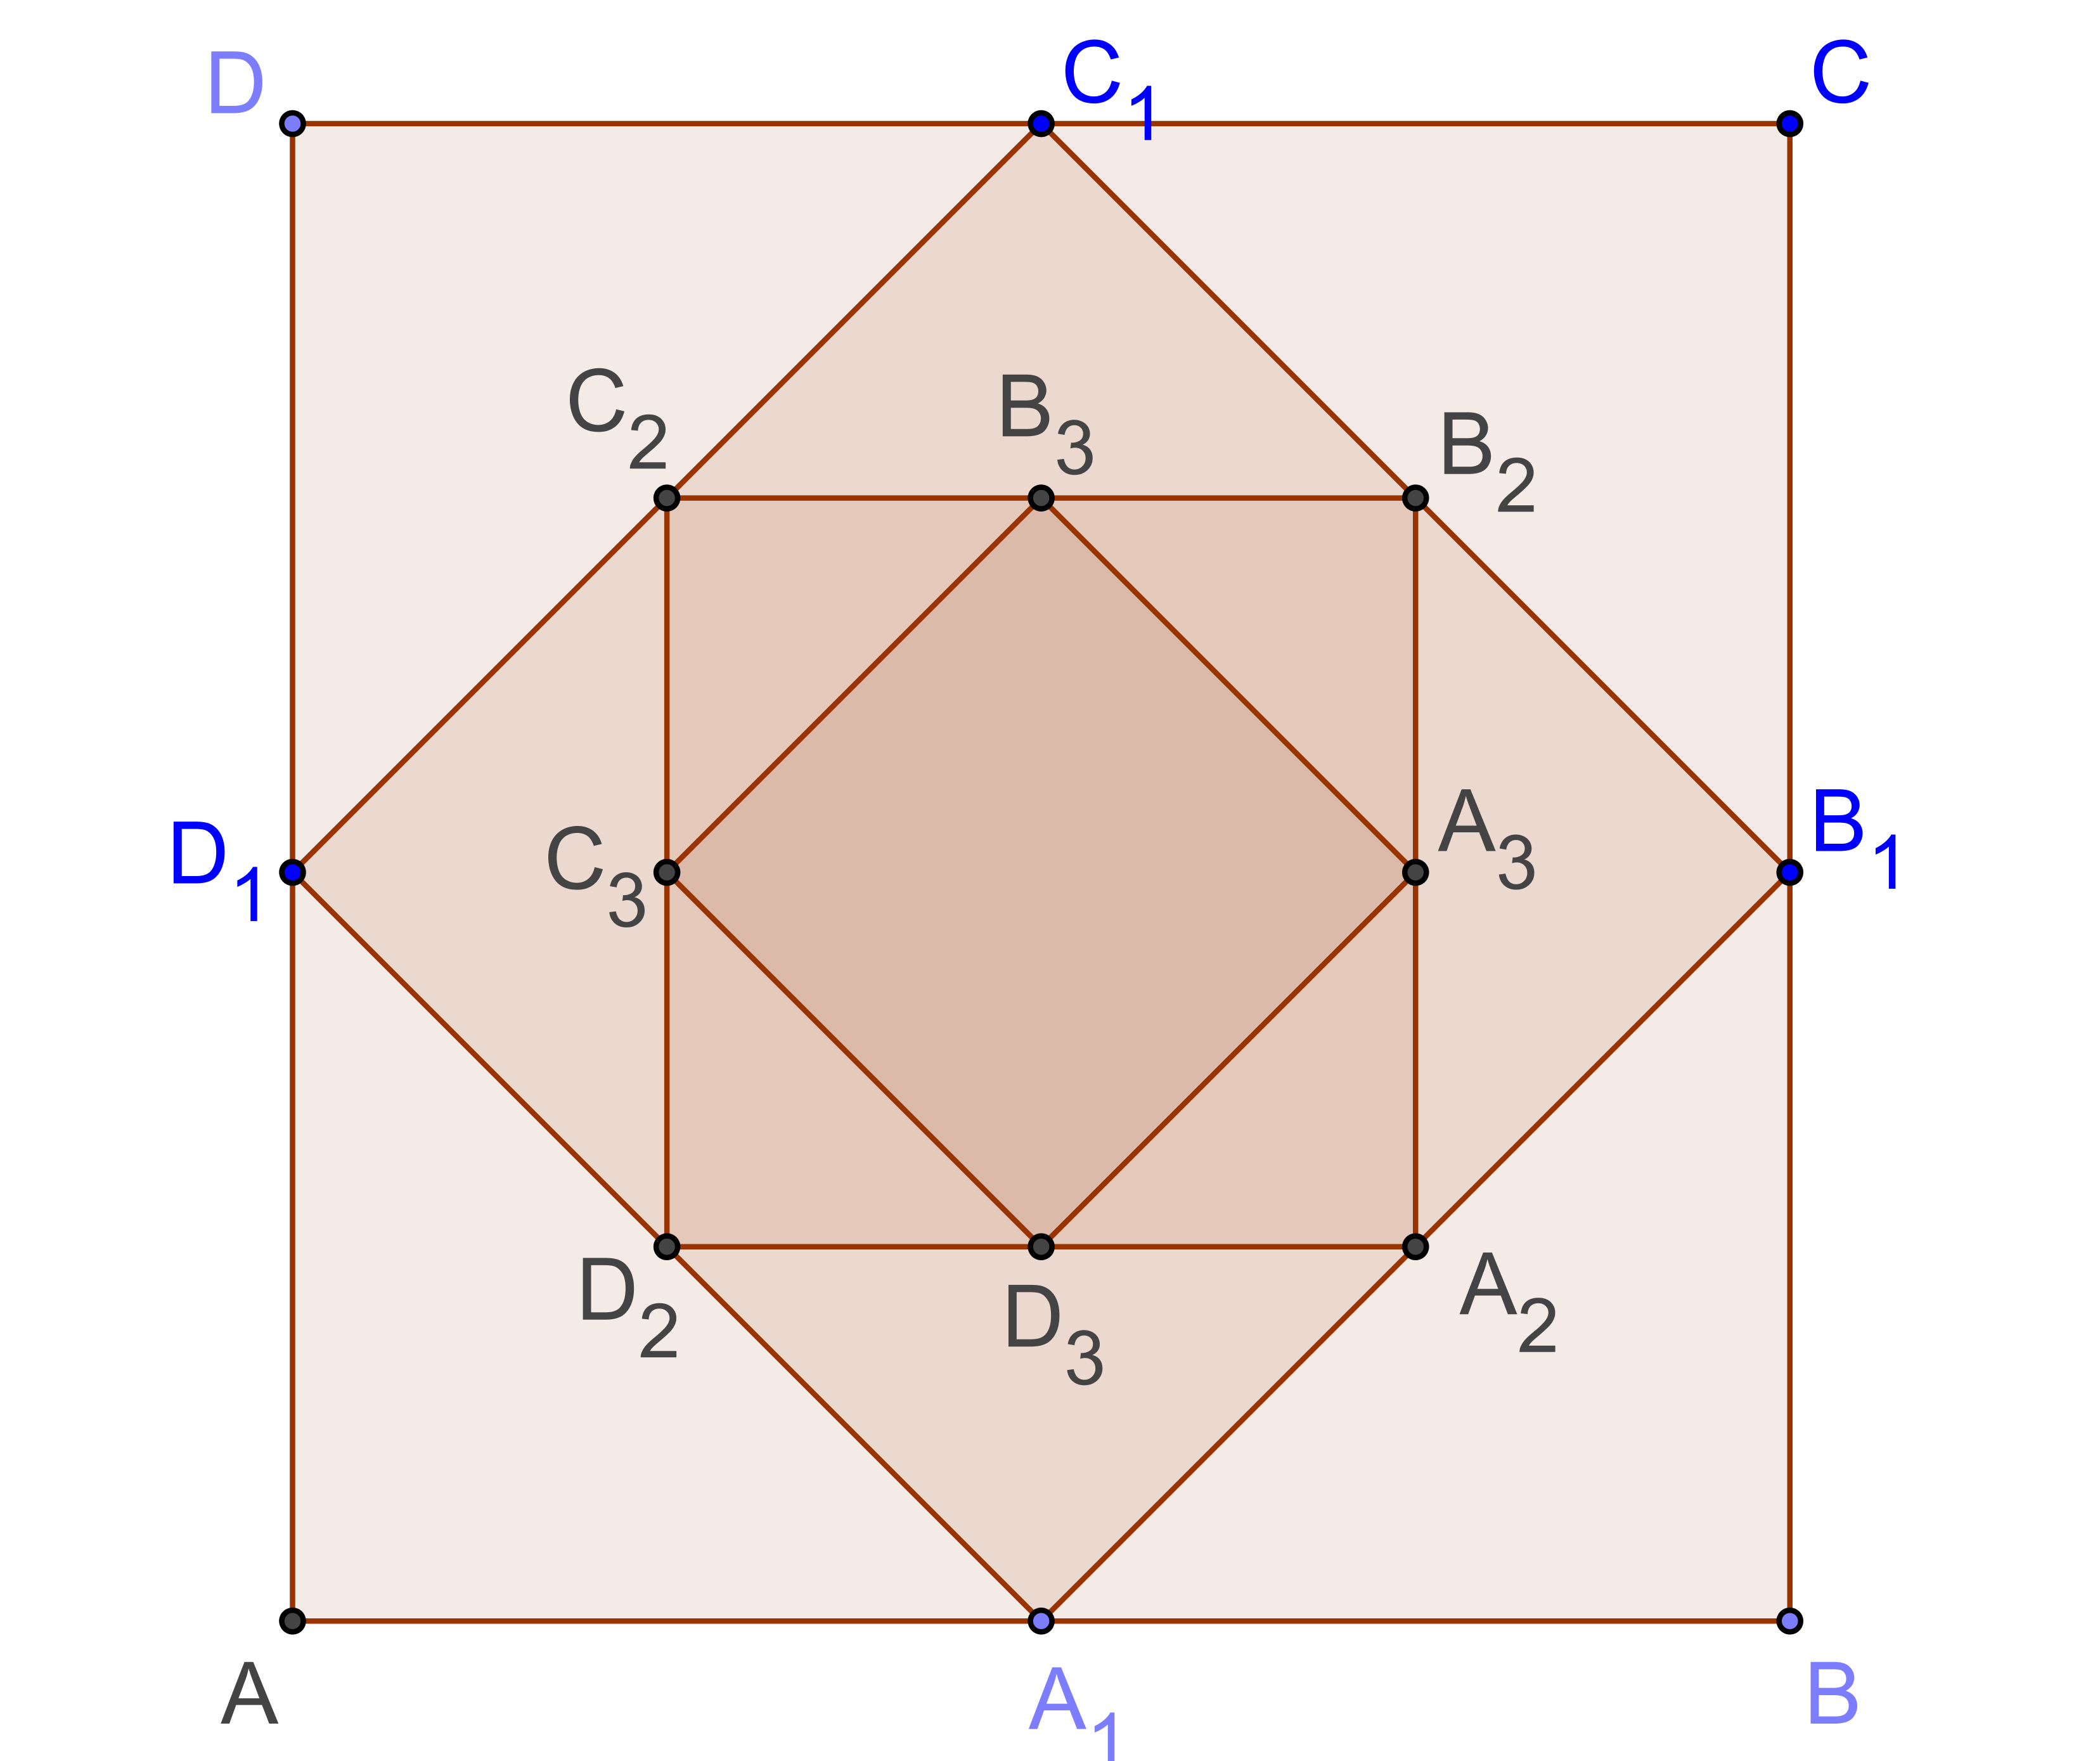
\includegraphics[width=0.5\textwidth]{30}
\end{figure}

\begin{mdframed}
\textbf{풀이 : }
\ov B{A_1}=1, \ov B{B_1}=1에서 \(\ov{A_1}{B_1}=\sqrt2\)이다.
따라서 \(S_1=(\sqrt2)^2=2\)이다.
또, \(\ov{B_1}{A_2}=\frac1{\sqrt2}\), \(\ov{B_1}{B_2}=\frac1{\sqrt2}\)에서 \(\ov{A_1}{B_1}=1\)이다.
따라서 \(S_2=1^2=1\)이다.
마찬가지로 계산하면 \(S_3=\frac12\), \(S_4=\frac14\) 등이다.
그러므로 수열 \(\{S_n\}\)은 첫항이 \(2\)이고 공비가 \(\frac12\)인 등비수열이다.
일반항을 계산하면
\[S_n=2\times\left(\frac12\right)^{n-1}=2\times2^{1-n}=2^{2-n}\]
이 된다.
따라서 
\begin{align*}
S_n 		&<0.01\\
2^{2-n}	&<\frac1{100}\\
2^{n-2}	&>100
\end{align*}
에서, \(n\)의 최솟값은 \(9\)이다.
\end{mdframed}

{\par
\raggedleft\textbf{답 : (\qquad\qquad\(n=9\)\qquad\qquad)}
\par}\bigskip\bigskip

%%
\section{등비수열의 활용}
%
\prob{}
아래 그림과 같이 한 변의 길이가 \(4\)인 정삼각형 \(ABC\)에서 \(AB\)의 중점을 \(A_1\), \(BC\)의 중점을 \(B_1\), \(CA\)의 중점을 \(C_1\)이라고 하고, 정삼각형 \(A_1B_1C_1\)의 넓이를 \(S_1\)이라고 하자.
또 \(A_1B_1\)의 중점을 \(A_2\), \(B_1C_1\)의 중점을 \(B_2\), \(C_1A_1\)의 중점을 \(C_2\)라고 하고, 정삼각형 \(A_2B_2C_2\)의 넓이를 \(S_2\)라고 하자.
이와 같은 과정을 반복하여 수열 \(\{S_n\}\)을 만들 때, \(S_5\)의 값을 구하시오.
(단, 한 변의 길이가 \(a\)인 정삼각형의 넓이는 \(\frac{\sqrt3}4a^2\)이다.)

\begin{figure}[h!]
\center
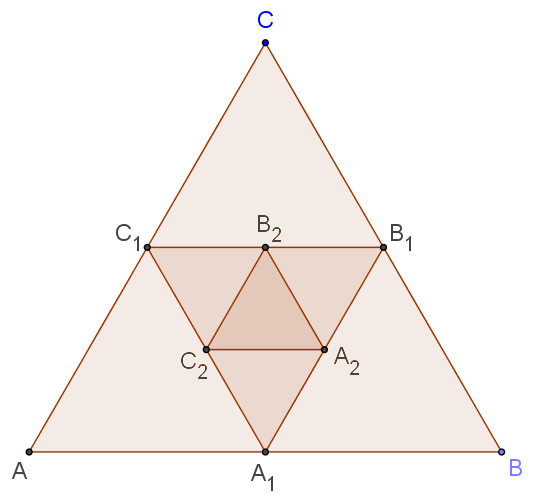
\includegraphics[width=0.5\textwidth]{31}
\end{figure}

\begin{mdframed}
\textbf{풀이 : }
\vspace{0.33\textheight}
\end{mdframed}
\ans

\clearpage

%
\exam{예금}\label{deposit_example_1}
연이율이 10\%인 은행에 100만 원을 예금한다고 하자.
1년 후에 받을 수 있는 돈은 원래 맡겨놓았던 100만 원과 이자인
\[100만 원\times\frac{10}{100}=10만 원\]
을 합친 금액인 110만 원이 된다.

%%
%\defi{이율, 원금, 이자, 원리합계}
%위의 예에서 원래 맡겨놓았던 금액인 100만 원을 \textbf{원금}이라고 하고, 늘어난 금액을 \textbf{이자}라고 한다.
%이자가 붙는 비율인 10\%는 \textbf{이율}이라고 부르며, \(r\)로 쓴다.
%위의 예에서 \(r=\frac{10}{100}=0.1\)이다.
%또한 원금과 이자를 합친 금액을 \textbf{원리합계}라고 한다.
%위의 예에서 원리합계는 110만 원이다.

%
\defi{원금, 이자, 원리합계, 이율}
은행에 돈을 맡길 때, 원래 맡겨놓은 금액을 \textbf{원금}, 늘어난 금액을 \textbf{이자}라고 한다.
원금과 이자를 합친 금액은 \textbf{원리합계}라고 부르며, 이자가 붙는 비율인 10\%는 \textbf{이율}이라고 부른다.
이율은 보통 \(r\)로 쓰며, 이율에는 연이율, 월이율 등이 있다.
위의 예에서
\begin{align*}
원금&=100만 원\\
이자&=10만 원\\
원리합계&=110만 원\\
이율&=r=\frac{10}{100}=0.1
\end{align*}

%
\exam{}\label{deposit_example_2}
예시 \ref{deposit_example_1}에서 2년 후에 받을 수 있는 돈은 얼마일까?
다음 두 가지의 방법을 생각해볼 수 있다.
\begin{enumerate}
\item
원금은 100만 원이었으니, 추가로 받을 수 있는 이자는 여전히 10만 원이다.
따라서 원리합계는 \(100+10+10=120\)만 원이다.
\item
1년 후에는 통장에 \(110\)만 원이 있으니, 추가로 받을 수 있는 이자는 \(110\times0.1=11\)만 원이 된다.
따라서 원리합계는 \(100+10+11=121\)만 원이다.
\end{enumerate}

\clearpage
%
\defi{예금, 단리, 복리}
원금을 일정한 기간동안 은행에 맡기는 것을 \textbf{예금}이라고 한다.
이때 원리합계를 구하는 방법은 두 가지로, 예시 \ref{deposit_example_2}의 (1)과 같은 방법을 \textbf{단리}, (2)와 같은 방법을 \textbf{복리}라고 한다.

\begin{figure}[h!]
\centering
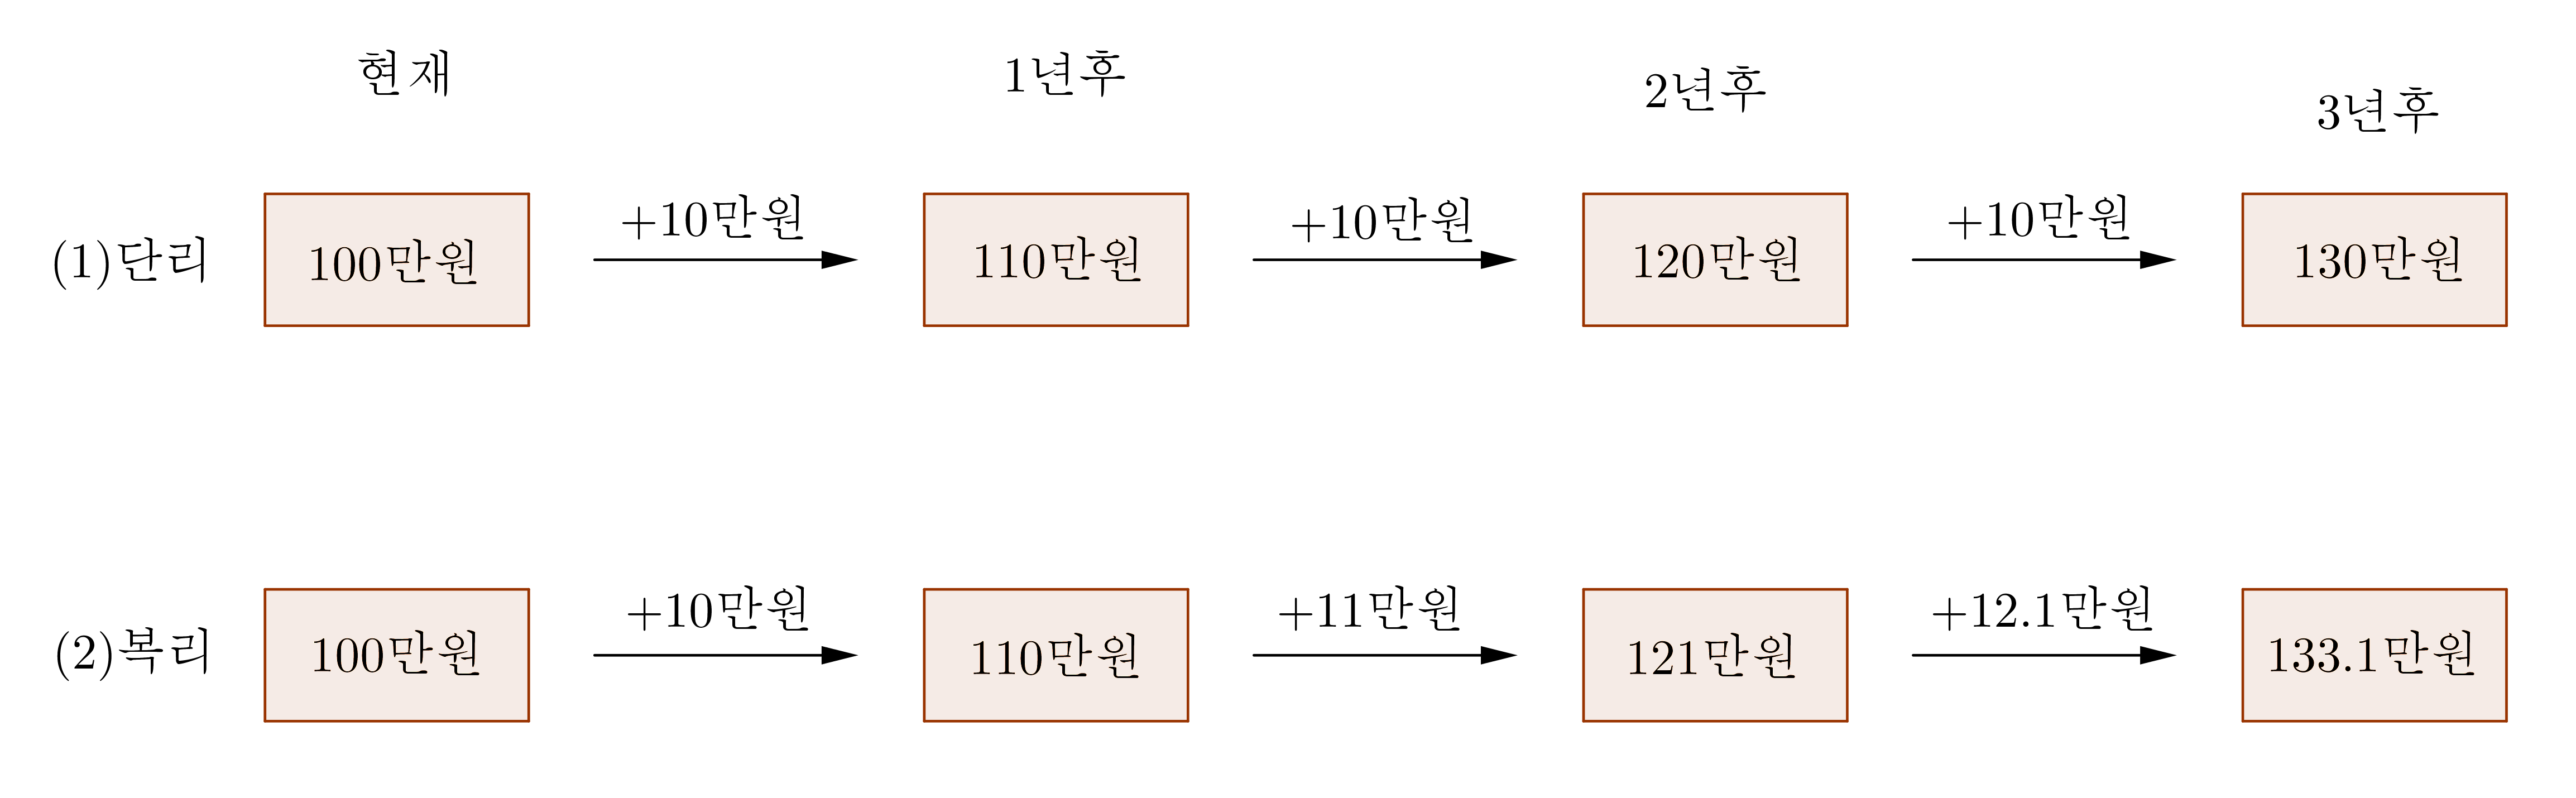
\includegraphics[width=0.8\textwidth]{34}
\end{figure}

%
\prob{}
원금 10만 원을 연이율 \(6\%\)로 예금할 때, 10년 후의 원리합계를 단리법, 복리법으로 각각 구하여라.
(단, \(1.06^{10}=1.79\)로 계산한다.)

\begin{mdframed}
\textbf{풀이 : }
\vspace{0.35\textheight}
\end{mdframed}
\ans

\end{document}